%% LyX 2.2.3 created this file.  For more info, see http://www.lyx.org/.
%% Do not edit unless you really know what you are doing.
\documentclass[oneside,english]{extbook}
\usepackage{lmodern}
\renewcommand{\sfdefault}{lmss}
\renewcommand{\ttdefault}{lmtt}
\usepackage[T1]{fontenc}
\usepackage[latin9]{inputenc}
\usepackage{geometry}
\geometry{verbose,tmargin=25mm,bmargin=25mm,lmargin=25mm,rmargin=25mm}
\setcounter{secnumdepth}{3}
\setcounter{tocdepth}{3}
\setlength{\parindent}{0bp}
\usepackage{babel}
\usepackage{float}
\usepackage{graphicx}
\usepackage{setspace}
\onehalfspacing
\usepackage[unicode=true,pdfusetitle,
 bookmarks=true,bookmarksnumbered=false,bookmarksopen=false,
 breaklinks=false,pdfborder={0 0 1},backref=false,colorlinks=false]
 {hyperref}

\makeatletter
%%%%%%%%%%%%%%%%%%%%%%%%%%%%%% User specified LaTeX commands.
\usepackage{amssymb}
\usepackage{color}
\usepackage{listings}
\definecolor{hellgelb}{rgb}{1,1,0.85}
\definecolor{colKeys}{rgb}{0,0,1}
\definecolor{colIdentifier}{rgb}{0,0,0}
\definecolor{colComments}{rgb}{1,0,0}
\definecolor{colString}{rgb}{0,0.5,0}
\lstset{
      language=Matlab,
      float=hbp,
      basicstyle=\footnotesize\ttfamily,
      identifierstyle=\color{colIdentifier},
      keywordstyle=\color{colKeys},
      stringstyle=\color{colString},
      commentstyle=\itshape\color{colComments},
      columns=fixed,
      tabsize=4,
      frame=single,
      framerule=1pt,
      extendedchars=true,
      showspaces=false,
      showstringspaces=false,
      numbers=left,
      numberstyle=\tiny\ttfamily,
      numbersep=1em,
      breaklines=true,
      breakindent=10pt,
      backgroundcolor=\color{hellgelb},
      breakautoindent=true,
      captionpos=t,
      xleftmargin=1em,
      xrightmargin=\fboxsep
}
\usepackage{lscape}
\usepackage{amsmath}
\usepackage{pifont}
\usepackage{color}

\delimitershortfall=-1pt
\let\Right\right
\let\Left\left
\makeatletter
\def\right#1{\Right#1\@ifnextchar){\!\right}{}}
\def\left#1{\Left#1\@ifnextchar({\!\left}{}}
\makeatother

\makeatother

\begin{document}
\pagenumbering{gobble}

\begin{figure}[H]
\centering\includegraphics[clip,scale=0.75]{../FIGURES/fig01}
\end{figure}

This lecture is about the simultaneous localization and mapping algorithm,
which is the topic that gives name to this course.\\

\begin{figure}[H]
\centering\includegraphics[clip,scale=0.75]{../FIGURES/fig02}
\end{figure}

Let's have a look at what we have done so far. Here's the robot at
a given position having a certain orientation and we know that there
is some uncertainty (error) associated to its position and orientation.
The uncertainty in the robot's position, $\left( x_t, \, y_t \right)$,
is expressed with an ellipse, $\Sigma_t$, while the uncertainty in
the robot's orientation, $\theta_t$, is expressed with a circular
sector, $\pm \, \sigma_{\theta_t}$. Now, the robot moves and the
inaccuracies in the movement induce an increase in the uncertainty
of the robot's pose. After the robot's motion the EKF algorithm calculates
the predicted pose for the robot, $\vec{\overline{\mu}}_t \, = \, \left( \overline{\mu}_{x_t}, \, \overline{\mu}_{y_t}, \, \overline{\mu}_{\theta_t}  \right)$,
aka, $\vec{\widetilde{x}}_t$. If the robot goes on moving and the
algorithm only carries out the prediction step, the uncertainty associated
to the position and orientation will increase continuously. But fortunately
there are some landmarks in the scene with \textbf{known positions}
and by measuring distances and bearings to those well-positioned landmarks
the algorithm is able to correct the pose for the robot. This correction
step also decrease the uncertainty associated to the position and
orientation for the robot. Again, until this lecture, to perform the
correction step it is essential that the landmarks' coordinates are
known in advance, and with that data the EKF algorithm, or the PF
algorithm, can resolve the localization problem.

\begin{figure}[H]
\centering\includegraphics[clip,scale=0.75]{../FIGURES/fig03}
\end{figure}

What happens if you don't know the positions of the landmarks in advance?
This is actually the usual case, because it is very hard to get hold
of cadastral maps or floor plans and even if you manage to do so you
will often notice that they are not very useful for localization because
the buildings have been built in a different way or they have been
modified later on or there are so many additional items like chairs
and tables, that are not part of the map, but modify a huge portion
of what the robot sees. 

Let's think about the following. The robot is somewhere and since
there isn't a map of landmarks the algorithm will have to produce
that map on its own. Since the algorithm starts with an empty map
it can define the robot's position in the map origin, $\left(0, \, 0\right)$,
and define the orientation along the x-axis, $\left( 0^{\circ} \right)$.
Besides, it can consider the uncertainty in position and heading angle
as 0. From the pose occupied by the robot, the robot's laser scanner
measures the distance and the bearing to each landmark within its
range of view. The algorithm can use all those pair of measurements
to define the landmarks' positions in the real world, i.e, in the
world that has its origin in the starting position of the robot. It
has to be noted that the defined landmarks are oriented along the
heading angle of the robot at the starting position. Having defined
those landmarks the algorithm will do the same as it did in the previous
lectures. Therefore, the robot moves along, the algorithm carries
out the prediction step, the uncertainty for the position and heading
angle of the robot increases, then the laser scanner get some landmark
observations (distance and bearing to each landmark within its range
of view) and finally the algorithm uses those measurements to correct
the position and orientation for the robot and get a smaller uncertainty
ellipse for the position and a smaller circular sector for the heading
angle. Instead of taking the landmarks from a map, which was obtained
by some external means, the algorithm takes the following steps:

Whenever the algorithm recognizes a landmark for the first time it
determines its position, relative to the map which it currently builds
up, and after that this landmark can be used for the localization
of the robot at all subsequent poses where that landmark is observed
again by the laser scanner, i.e, whenever that landmark is within
the range of view of the laser. Well, it is not exactly as easy as
that because when the algorithm recognises a landmark for the first
time the measurement of the distance and bearing to the landmark induces
an uncertainty (error) in the landmark's position. What becomes clear
is that the algorithm can't simply put a landmark into the map when
it recognizes the landmark for the first time and then to assume that
the landmark's position is correct. When the algorithm recognizes
a landmark for the first time it puts that new landmark into the map
with a certain uncertainty in position. Then, every time the laser
scanner takes a scan that contains a measurement for that landmark
(distance and bearing) the algorithm updates the landmark's position
and reduces its uncertainty in position. This is the same process
that the algorithm carries out with the robot's pose.

In the previous EKF implementation, the system state was the robot's
pose, i.e, its position and heading angle. Now, in the SLAM algorithm
the system state comprises the robot's pose and the positions of the
landmarks that the algorithm finds (coordinate $x_{L_k}$ and coordinate
$y_{L_k}$ of each found landmark). What you see now, immediately,
is that the state vector doesn't have a constant size anymore. For
each landmark that the algorithm observes, and that it didn't observe
before, the state vector grows by two elements.\\
\begin{figure}[H]
\centering\includegraphics[clip,scale=0.75]{../FIGURES/fig04}
\end{figure}

Let's consider that the robot starts in the pose $(0, \, 0, \, 0^{\circ})$
with a large uncertainty in position and heading angle. Later on the
robot observes some landmarks and since the uncertainty for its pose
is large the uncertainty ellipses for those landmarks will be large
too. The robot moves and observes those landmarks again, so all those
uncertainty ellipses will get a bit smaller. Let's consider that the
robot moves for a real long time in the environment, observing those
landmarks over and over again. Therefore, my hope is that those uncertainty
ellipses get smaller and smaller until they are really really small
so that the landmarks are not uncertain anymore. So that this situation
is equivalent to what we had earlier, in the EKF approach, where the
landmarks were assumed to be error-free. What do you think? Will the
uncertainty in the landmarks' positions go down to zero as the number
of measurements goes to infinity?

\begin{figure}[H]
\centering\includegraphics[clip]{../FIGURES/fig06}
\end{figure}

\begin{figure}[H]
\centering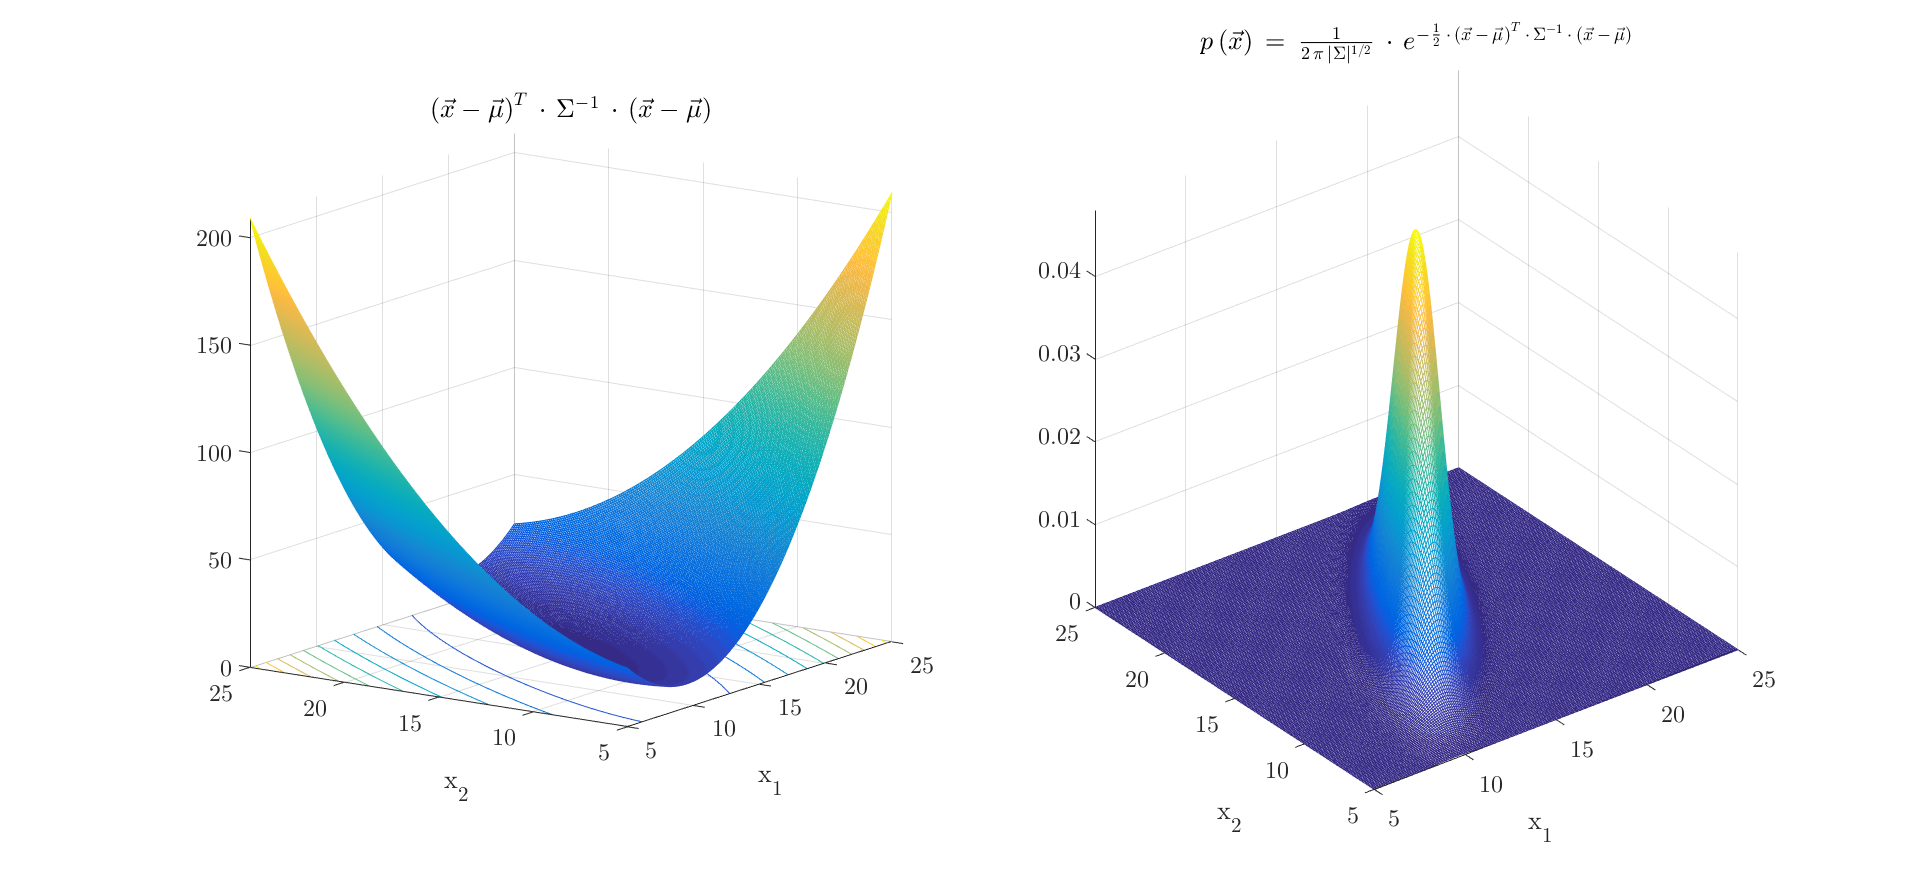
\includegraphics[clip]{../FIGURES/fig08}
\end{figure}

\begin{figure}[H]
\centering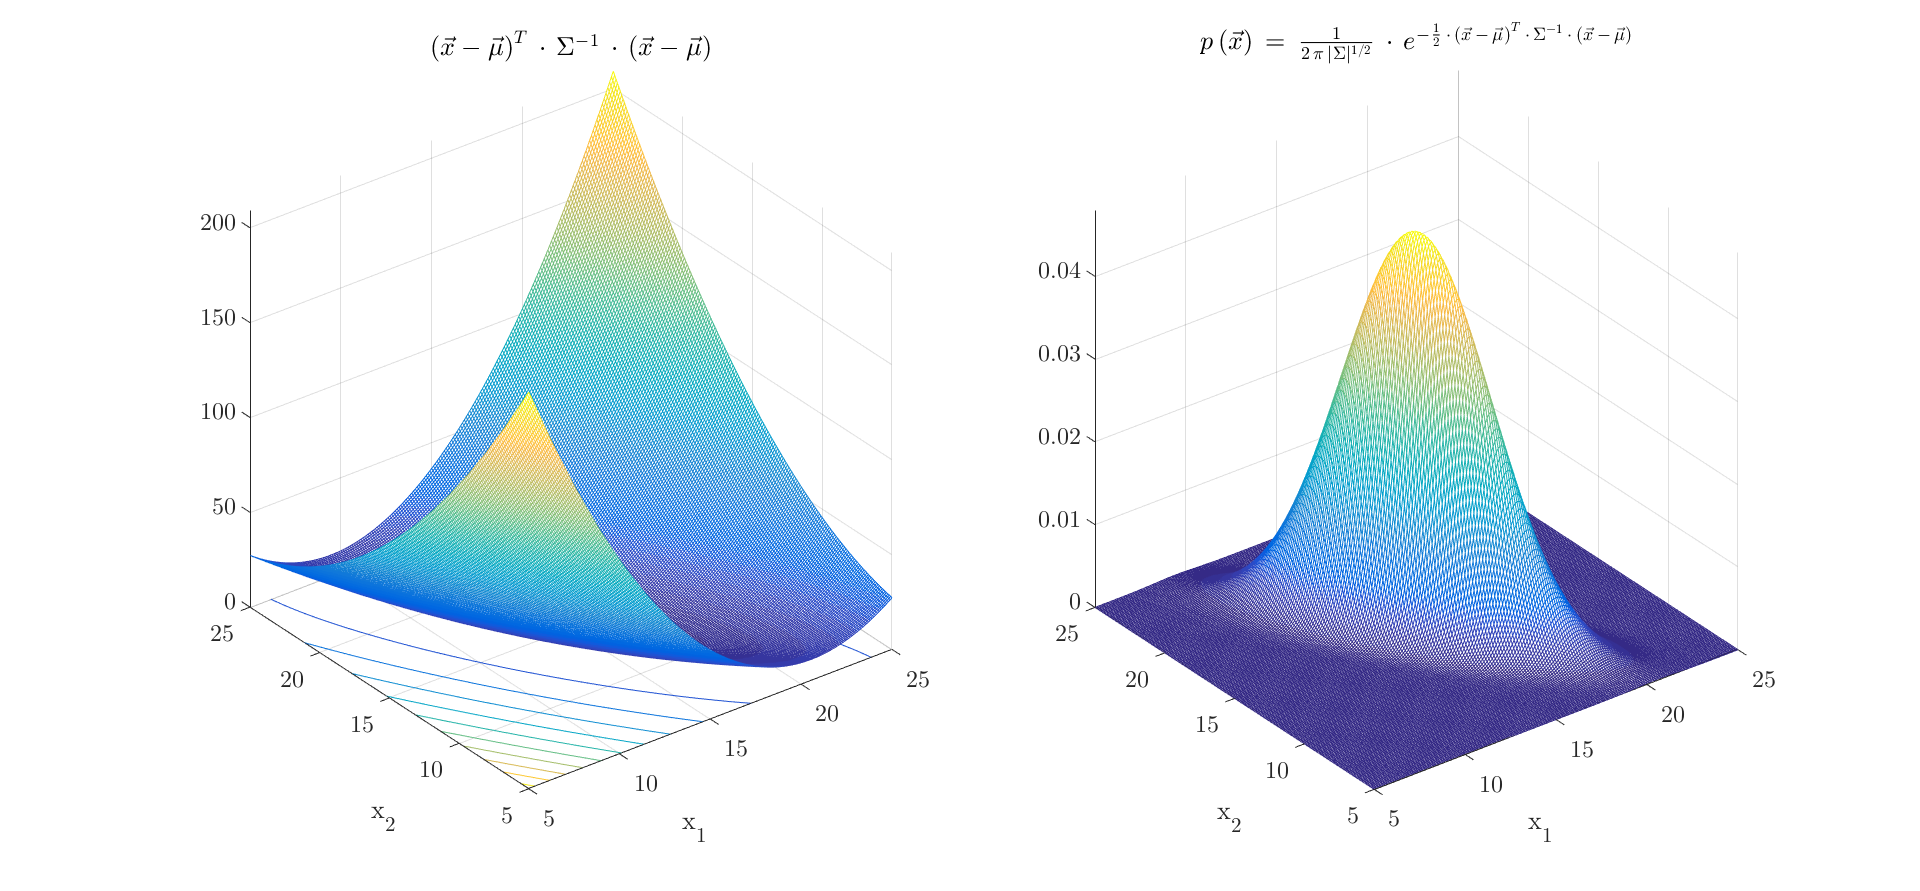
\includegraphics[clip]{../FIGURES/fig10}
\end{figure}

\end{document}
